\chapter{Metodologie di riconoscimento delle gesture}
\label{chap:metodi}

Come già specificato in \ref{intro}, il framework mette a disposizione due collezioni distinte di punti tridimensionali: 
\begin{itemize}
    \item la lista dei landmark a coordinate globali con origine nel centro geometrico approssimato della mano
    \item la lista dei landmark con coordinate X e Y normalizzate all'intervallo [0.0 - 1.0] per le dimensioni dell'immagine in input, la coordinata Z trova il suo centro nella posizione del landmark del polso
\end{itemize}

\noindent Abbiamo utilizzato entrambe le strutture per la rilevazione delle gesture, insieme a una combinazione delle le tecniche descritte di seguito, impiegando l'una o l'altra a seconda del tipo di azione alla quale la particolare gesture è collegata (vedi \ref{gesture}).

\section{Distanze tra landmark}

Il primo metodo che abbiamo implementato per discriminare una gesture dall'altra consiste semplicemente nel considerare la distanza tra landmark impiegando un sottoinsieme di punti rilevanti per la particolare gesture.

Abbiamo rilevato le distanze tra landmark caratterizzanti una particolare posizione delle dita che forma la gesture voluta in modo empirico, sfruttando opportune stringhe di log per visualizzare in tempo reale le distanze dei punti, per poi compilare una struttura dati usata come riferimento per identificare la gesture.

In seguito a queste analisi abbiamo notato, come ipotizzato in precedenza, le piccole ma non trascurabili fluttuazioni dei valori ottenuti dal framework, che impedivano un accurato riconoscimento della gesture; questo ha portato a considerare una soglia di errore sulle distanze rilevate, effettivamente individuando dei range di posizionamento delle dita che costituivano le gesture.

Aggiungendo nuove gesture alla nostra applicazione, abbiamo riscontrato un livello di inaccuratezza sempre più alto, manifestato nella forma di gesture rilevate contemporaneamente ad altre o, in certi casi, non rilevate affatto.

\section{Normalizzazione a livelli}

Dati i risultati della prima fase di test, abbiamo realizzato che molti fallimenti nella rilevazione di una gesture erano dovuti alla naturale differenza di dimensione tra le nostre mani.

Il passo successivo è stato quindi quello di trovare un modo per tentare di normalizzare le misure effettuate, questo ci ha portato a identificare, dopo una serie di prove, una distanza caratteristica da utilizzare come misura per uniformare le altre. Accordando sulla misura della distanza dalla punta del dito medio al landmark del polso, siamo riusciti a migliorare nettamente il riconoscimento di una determinata gesture effettuate da mani differenti.

Questa distanza è calcolata sommando le distanze tra i quattro landmark del dito medio (le tre falangi e la base) e la distanza tra la base e il landmark polso.

Abbiamo poi accoppiato questa tecnica con la mappatura delle misure a un range di livelli discreto, in modo da ridurre l'impatto dell'instabilità dei valori forniti dal framework, a scapito di un minimo livello di accuratezza, dopo diversi tentativi, abbiamo deciso di suddivedere la distanza scelta in 70 livelli, valore che ritiene una precisione sufficiente delle misure e mitiga gli effetti delle fluttuazioni.

\section{Lo spazio tridimensionale}

Le tecniche implementato fino ad ora non tengono veramente conto del fatto che le gesture hanno una forte caratteristica tridimensionale, in quanto riducono lo stato della mano a un insieme di parametri monodimensionali, abbiamo infatti notato che molte posizioni che vogliamo identificare presentano notevoli similitudini nello spazio delle distanze tra landmark.

Un parametro che abbiamo scelto di adottare nel sistema di riconoscimento è quello dell'allineamento nello spazio tridimensionale di un certo dito, o più in generale di un insieme di landmark.

Per ottenere questa informazione, abbiamo implementato una serie di funzioni di utilità che permettono di identificare il discostamento che una serie di punti ha dalla retta 3D formata da altri due punti dati; il calcolo di questa misura, unito a una lista di valori di errore ottenuti in modo sperimentale, permette di quantificare il livello di ripiegamento di un certo dito.

\begin{figure}[H]
    \caption{caption}
    \centering
    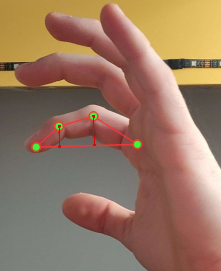
\includegraphics[width=0.5\textwidth]{/home/riccardoob/RelazioneSisDig/chapters/RelazioneSisDig/images/mano_vettore.png}
\end{figure}

Grazie a questa tecnica, unita alle metodologie sopra descritte, siamo riusciti a ottenere una identificazione molto più accurata della posizione delle dita di una mano e a ridurre significativamente il grado di sovrapposizione tra gesture.

Anche in questo caso abbiamo implementato la normalizzazione a livelli delle misure effettuate, prendendo però in considerazione una distanza di riferimento variabile, ovvero la lunghezza di ogni falange del dito considerato.

\section{Rilevamento velocità e direzione}

L'utilità di un sistema di riconoscimento di gesture non si ferma soltanto alla rilevazione di posizioni statiche, è infatti desiderabile poter ottenere anche informazioni relative alla velocità e direzione di certi landmark significativi, utilizzando poi questi dati per abilitare l'utente a una gamma più vasta di interazioni.

Per una delle gesture implementate, si è reso necessario creare una apposita classe \texttt{TimedPoint}, che mette a disposizione funzionalità di calcolo della velocità media e della direzione tra due \texttt{TimedPoint}, questi dati vengono poi utilizzati per abilitare l'identificazione di gesture in seguito a un movimento definito a una certa velocità media.

Questi calcoli ci hanno permesso di definire gesture \textbf{dinamiche}, che devono essere rilevate \textbf{in seguito a un movimento} effettuato a una certa velocità e in una certa direzione, e non in seguito all'avverarsi di una posizione statica.

E' importante specificare che anche le gesture cosiddette \textit{statiche}, in certi casi vengono utilizzate per ottenere parametri che vengono poi applicati in particolari modi all'applicazione, il fatto che questi parametri sono dinamici non le categorizza come gesture dinamiche. 


